\documentclass{exam}

\usepackage[spanish]{babel}
\usepackage[utf8]{inputenc}
\usepackage[T1]{fontenc}
\usepackage[newcommands]{ragged2e}
\usepackage{hyperref}
\usepackage{algorithm,algorithmic}
\usepackage{colortbl}
\usepackage{graphicx}
\usepackage{multicol}
\usepackage{enumitem}
\usepackage{float}
\usepackage{
  amsmath,
  amssymb,
  eso-pic,
  float,
  graphicx,
  lmodern,
  wrapfig,
  tabularx,
  multicol,
  multirow,
  color,
  colortbl,
  lastpage,
  titlesec,
  sectsty
}


\definecolor{azul}{RGB}{33,127,190}
\sectionfont{\color{azul}}
\subsectionfont{\color{azul}}
\renewcommand{\familydefault}{\sfdefault}

\footer{}{\thepage}{}

\makeatother

\title{\LARGE\color{azul}\textbf{Estructura de Datos - Certamen 2 }}
\author{\smallsize \color{gray}{Profesor: } \color{black}{\textbf{Eduardo Godoy}}}
\date{\normalsize \em \today}

\begin{document}

\AddToShipoutPictureBG*{%
  \AtPageUpperLeft{\raisebox{-\height}{
\includegraphics[scale=.95]{base/header.png}}}}

\maketitle

\begin{multicols}{2}
  \begin{flushleft}
    \textbf{Nombre:} \\
    \vspace*{2mm}
    \textbf{Rut:} \\
    \vspace*{2mm}
    \textbf{Paralelo:}
  \end{flushleft}
  \begin{center}
    \begin{table}[H]
      \begin{tabular}{p{4cm}|p{3cm}|}
        \arrayrulecolor{gray!50}\cline{2-2} ~ & {\em {\scriptsize \color{gray!50}{Puntaje:}}}\\
         & ~ \\
         ~ & \textbf{Nota:}
        \\ & ~ \\
        \arrayrulecolor{gray!50}\cline{2-2}
      \end{tabular}
    \end{table}
  \end{center}
\end{multicols}

%\vspace*{-18mm}
\noindent
\textbf{\\Instrucciones:}
\begin{itemize}
\item[-] El puntaje máximo  es 100 puntos.
\item[-] Tiempo máximo: 120 minutos.
\item[-] El certamen es \underline{\textbf{individual}}. Cualquier intento de copia, será sancionado según dicta el reglamento de la carrera.
\end{itemize}

\noindent
\textbf{Resultados de aprendizaje a evaluar:}
\begin{enumerate}
\item Conocer e Implementar algoritmos para grafos y árboles  estructuras de datos complejas.
\vspace{2mm}

\noindent
\textbf{Contenido:} Este certamen evalúa los siguientes temas:

\vspace{-2mm}
\begin{table}[H]
  \begin{tabular}{
    !{\color{gray!50}\vrule}l
    !{\color{gray!50}\vrule}c
    !{\color{gray!50}\vrule}c
    !{\color{gray!50}\vrule}} \arrayrulecolor{gray!50} \hline
    \multicolumn{1}{!{\color{gray!50}\vrule}c}{\multirow{2}{*}{\textbf{
    Tema
    }}} &
          \multicolumn{2}{!{\color{gray!50}\vrule}c!{\color{gray!50}\vrule}}{\textbf{
          Puntajes
          }} \\ \arrayrulecolor{gray!50}\cline{2-3} &
                                                      \multicolumn{1}{!{\color{gray!50}\vrule}c!{\color{gray!50}\vrule}}{\textbf{
                                                      Total
                                                      }} &
                                                           \multicolumn{1}{c!{\color{gray!50}\vrule}}{\textbf{
                                                           Obtenido
                                                           }} \\ \arrayrulecolor{gray!50} \hline
    Problema 1: Conocimiento de estructuras de datos gerarquicas
        & \multicolumn{1}{!{\color{gray!50}\vrule}c!{\color{gray!50}\vrule}}{\textbf{
          40 pts.
          }} & \\ \arrayrulecolor{gray!50} \hline
    Problema 2: Creación y Recorrido de árboles
        & \multicolumn{1}{!{\color{gray!50}\vrule}c!{\color{gray!50}\vrule}}{\textbf{
          20 pts.
          }} & \\ \arrayrulecolor{gray!50} \hline
          Problema 3: TDA - Algóritmos para recorrer Grafos.
              & \multicolumn{1}{!{\color{gray!50}\vrule}c!{\color{gray!50}\vrule}}{\textbf{
                40 pts.
                }} & \\ \arrayrulecolor{gray!50} \hline

  \end{tabular}
\end{table}

\newpage

\vspace{-7mm}
\section{\textbf{Problema 1}} \textbf{\emph{40pts.}}
\noindent
% \textbf{Plantamiento de problema: }
\begin{questions}
  \item \textbf{\emph{30pts.}} Dada las siguientes claves cree el árbol AVL desatallando lo siguiente:

  \begin{itemize}
    \item Valor a insertar en cada paso.
    \item Factor de equilibrio en cada sub arbol.
    \item Tipo de rotación aplicada.
  \end{itemize}

  \item \textbf{\emph{10pts.}} Sobre el árbol resultante aplique el recorrido Inorden.

  \begin{itemize}

    \begin{table}[H]
    \centering
    \begin{tabular}{|l|l|l|l|l|l|l|l|l|l|l|}
    \hline
      18 & 14 & 15 & 19 & 20 & 21 & 7 & 4 & 2 & 5 & 6 \\
    \hline
    \end{tabular}
    \end{table}

  \end{itemize}

\end{questions}

\begin{table}[H]
  \centering
  \begin{tabular}{
    !{\color{gray!50}\vrule}p{3.9cm}
    !{\color{gray!50}\vrule}p{3.6cm}
    !{\color{gray!50}\vrule}p{3.6cm}
    !{\color{gray!50}\vrule}p{3.6cm}
    !{\color{gray!50}\vrule}} \arrayrulecolor{gray!50} \hline
    \multicolumn{4}{!{\color{gray!50}\vrule}c!{\color{gray!50}\vrule}}{\textbf{¿Cómo  seré evaluado en este trabajo?}} \\ \arrayrulecolor{gray!50}
    \hline
    %
    \textbf{Ítem} & \textbf{Logrado} & \textbf{Suficiente} & \textbf{No Logrado}\\ \arrayrulecolor{gray!50} \hline\newline
    Pregunat 1 - Inserción: &
    Inserta  Valor de forma corresta: 5 pts   &
    Inserta valor  parcialmente: 0pts  &
    AInserta Valor de forma incorrecta: 0pts \\ \arrayrulecolor{gray!50} \hline

    Pregunat 1 - Factor de equilibrio. &
    Calcula de forma correcta: 10pts   &
    Calcula parcialmente: 5pts  &
    Calcula de forma incorrecta: 0pts \\ \arrayrulecolor{gray!50} \hline

    Pregunat 1 - Rotaciones. &
    Aplica de forma correcta 15pts   &
    Aplica parcialmente 5pts &
    Aplica de forma incorrecta  0pts\\ \arrayrulecolor{gray!50} \hline

    Pregunat 1 - Recorrido. &
    Aplica de forma correcta 10pts   &
    Aplica parcialmente 5pts &
    Aplica de forma incorrecta  0pts\\ \arrayrulecolor{gray!50} \hline

    Total de la sección &  40pts & 15pts & 0pts\\ \arrayrulecolor{gray!50} \hline
  \end{tabular}
  \label{tbl:1}
\end{table}

\vspace{-5mm} \ textbf{Nota:} En caso de que el ítem no esté presente,
tiene ponderación cero.



\newpage
\vspace{-7mm}
\section{\textbf{Problema 2}}
\noindent
% \textbf{Plantamiento de problema: }

\begin{questions}

  \begin{enumerate}
  \item \textbf{\emph{20pts.}} Crear un árbol B insertado las siguientes claves:

  \begin{table}[H]
  \centering
  \begin{tabular}{|l|l|l|l|l|l|l|l|l|l|l|l|l|l|l|l|}
  \hline
    32&	5	&25&	8&	40&	10&	30&	15&	20&	31&	13&	11&	14&	33&	18&	17\\
  \hline
  \end{tabular}
  \end{table}

\begin{itemize}
  \item Considere a m=5.
  \item m-1 número de claves por cada hoja.
  \item (m-1)/2 = como el valor medio.
\end{itemize}

    \end{enumerate}
  \end{questions}

  \begin{table}[H]
    \centering
    \begin{tabular}{
      !{\color{gray!50}\vrule}p{3.9cm}
      !{\color{gray!50}\vrule}p{3.6cm}
      !{\color{gray!50}\vrule}p{3.6cm}
      !{\color{gray!50}\vrule}p{3.6cm}
      !{\color{gray!50}\vrule}} \arrayrulecolor{gray!50} \hline
      \multicolumn{4}{!{\color{gray!50}\vrule}c!{\color{gray!50}\vrule}}{\textbf{¿Cómo seré evaluado en este trabajo?}} \\ \arrayrulecolor{gray!50} \hline
      \textbf{Ítem} & \textbf{Logrado} & \textbf{Suficiente} & \textbf{No Logrado}\\ \arrayrulecolor{gray!50} \hline
      Conocimiento del algoritmo &
      Aplica de forma correcta el algoritmo 20 pts   &
      Aplica parcialmente con menos de 3 errores 10 pts  &
      Aplica de forma incorrecta con 4 errores o más 0pts\\ \arrayrulecolor{gray!50} \hline
      Total de la sección &  20pts & 10pts & 0pts\\ \arrayrulecolor{gray!50} \hline
    \end{tabular}
    \label{tbl:1}
  \end{table}
  \vspace{-5mm}
  \textbf{Nota:} En caso de que el {í}tem no est{é} presente, tiene ponderaci{ó}n cero.

  \newpage
  \vspace{-7mm}
  \section{\textbf{Problema 3}}
  \noindent
  \begin{questions}

    \begin{enumerate}

      \item \textbf{\emph{40pts.}} Dado el siguente grafo, aplicar el algoritmo de dijktra identificando el camino mas corto entre A y J:

      \begin{center}
          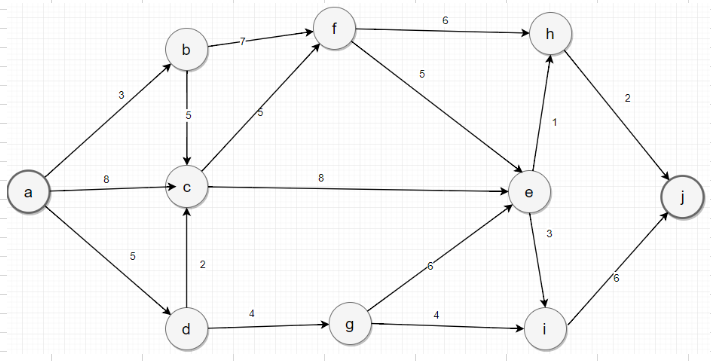
\includegraphics[width=.9\textwidth]{./img/grafo}
      \end{center}

     \end{enumerate}
  \end{questions}


    \begin{table}[H]
      \centering
      \begin{tabular}{
        !{\color{gray!50}\vrule}p{3.9cm}
        !{\color{gray!50}\vrule}p{3.6cm}
        !{\color{gray!50}\vrule}p{3.6cm}
        !{\color{gray!50}\vrule}p{3.6cm}
        !{\color{gray!50}\vrule}} \arrayrulecolor{gray!50} \hline
        \multicolumn{4}{!{\color{gray!50}\vrule}c!{\color{gray!50}\vrule}}{\textbf{¿Cómo seré evaluado en este trabajo?}} \\ \arrayrulecolor{gray!50} \hline
        \textbf{Ítem} & \textbf{Logrado} & \textbf{Suficiente} & \textbf{No Logrado}\\ \arrayrulecolor{gray!50} \hline
        \textbf{insertEnd}. &
        Aplica de forma correcta 40pts   &
        Aplica parcialmente con  3 errores 20pts  &
        Aplica de forma incorrecta 0pts\\ \arrayrulecolor{gray!50} \hline



        Total de la sección &  40pts & 20pts & 0pts\\ \arrayrulecolor{gray!50} \hline
      \end{tabular}
      \label{tbl:1}
    \end{table}
    \vspace{-5mm}
    \textbf{Nota:} En caso de que el {í}tem no est{é} presente, tiene ponderaci{ó}n cero.
\end{document}
